\documentclass[fontsize=24,
               ]{beamer}

% Language and encoding
\usepackage[english]{babel}
\usepackage[utf8]{inputenc}

% Bibliography and citation
%\usepackage[backend=biber]{biblatex}

% Colors
\usepackage{xcolor}
\selectcolormodel{cmyk}

% New colors
\definecolor{grey}{rgb}{0.5,0.5,0.5}
\definecolor{darkgrey}{rgb}{0.25,0.25,0.25}
\definecolor{brightgrey}{rgb}{0.75,0.75,0.75}
\definecolor{water}{rgb}{0.5,0.7,1}

% Images
\usepackage{caption}
\usepackage{subcaption}
\usepackage{placeins}
\usepackage{wrapfig}
\usepackage{tikz}
\usepackage{pgfplots}
\usepackage{adjustbox}
%\usepackage{environ}
\usetikzlibrary{arrows, calc}

% Configure tikz
%\tikzset{
%    x=0.1\textwidth,
%    y=0.1\textwidth,
%    }

% Configure captions
\renewcommand\thesubfigure{\arabic{subfigure}}

% Physics and maths
\usepackage{physics}
\usepackage{amsmath}
\usepackage{mathtools}
\usepackage{upgreek}
\usepackage{amssymb}
\usepackage[separate-uncertainty=true,
            list-units = single,
            list-separator = {;\,},
            exponent-product=\cdot,
            ]{siunitx}

% Poster specific
\usepackage[orientation=portrait,
            size=a0,
            scale=1.0,
            ]{beamerposter}
\usepackage[absolute,
            overlay,
            ]{textpos}
\setlength{\TPHorizModule}{1cm}
\setlength{\TPVertModule}{1cm}
\usetheme{Dreuw}

%bibliography
\bibliographystyle{plain}

% Title
\graphicspath{{../figures/}}
\title[Metamaterials]{Metamaterials}
\author[Sattler \& Marquardt]{Alexander Sattler \\ \& Michael Marquardt}
\institute[Universität Stuttgart]{Universität Stuttgart}
\date{18.06.2018}

% New commands for posters
\usepackage{varwidth}
\newcommand\Umbruch[2][0.15\linewidth]{
    \begin{varwidth}{#1}
        \flushleft #2   
    \end{varwidth}}
    \newenvironment{indentitemize}{%
        \begin{itemize}%
            \addtolength{\itemindent}{2ex}%
            \setlength{\leftmargin}{2ex}%
            \setlength{\topsep}{0pt}%
        }
        {%
        \end{itemize}%
    }

\newcommand*\circled[1]{\tikz[baseline=(char.base)]{\node[shape=circle,draw,inner sep=.4ex, line width = 1.5mm] (char) {#1};}}
\begin{document}

% Example using columns
\begin{frame}{}
\begin{columns}[t]

\begin{column}{0.48\linewidth}
    \begin{block}{\circled{1} Introduction}
        \textbf{Aim:}
\begin{itemize}
\item{Fabrication of split-ring resonators (SRRs) by using shadow nanosphere lithography}
\item{Analysing the spectral properties of the SRRs with FTIR}
\end{itemize}
\textbf{Motivation:}
\begin{itemize}
\item{Fast, cheap and large area fabrication technique}
\item{Tunable optical metamaterials resonance in the range of \SI{100}{THz}}
\end{itemize}

    \end{block}
    
     \begin{block}{\circled{2} Theory}
        Metamaterials are materials with a structure which is smaller then the wavelenght of ligth. The special properties of metamaterials is  based on the fact that they have a negative permeability $\mu$ and permittivity $\epsilon$. That leads to a negative refractive index $n = \sqrt{\epsilon \cdot \mu}$. 
The Lorentz-Oscillator model describes the optical characteristics of intraband  and the Drude model of the interband transitions and both can show  a negative $\epsilon$. The negative $\mu$ can be explained with the Kirchhoff's circuit laws. \\
The reflection spectrum of SRR shows frequency and polarisation dependencies \ref{spectrum_theory}.
\begin{figure}[H]
\centering
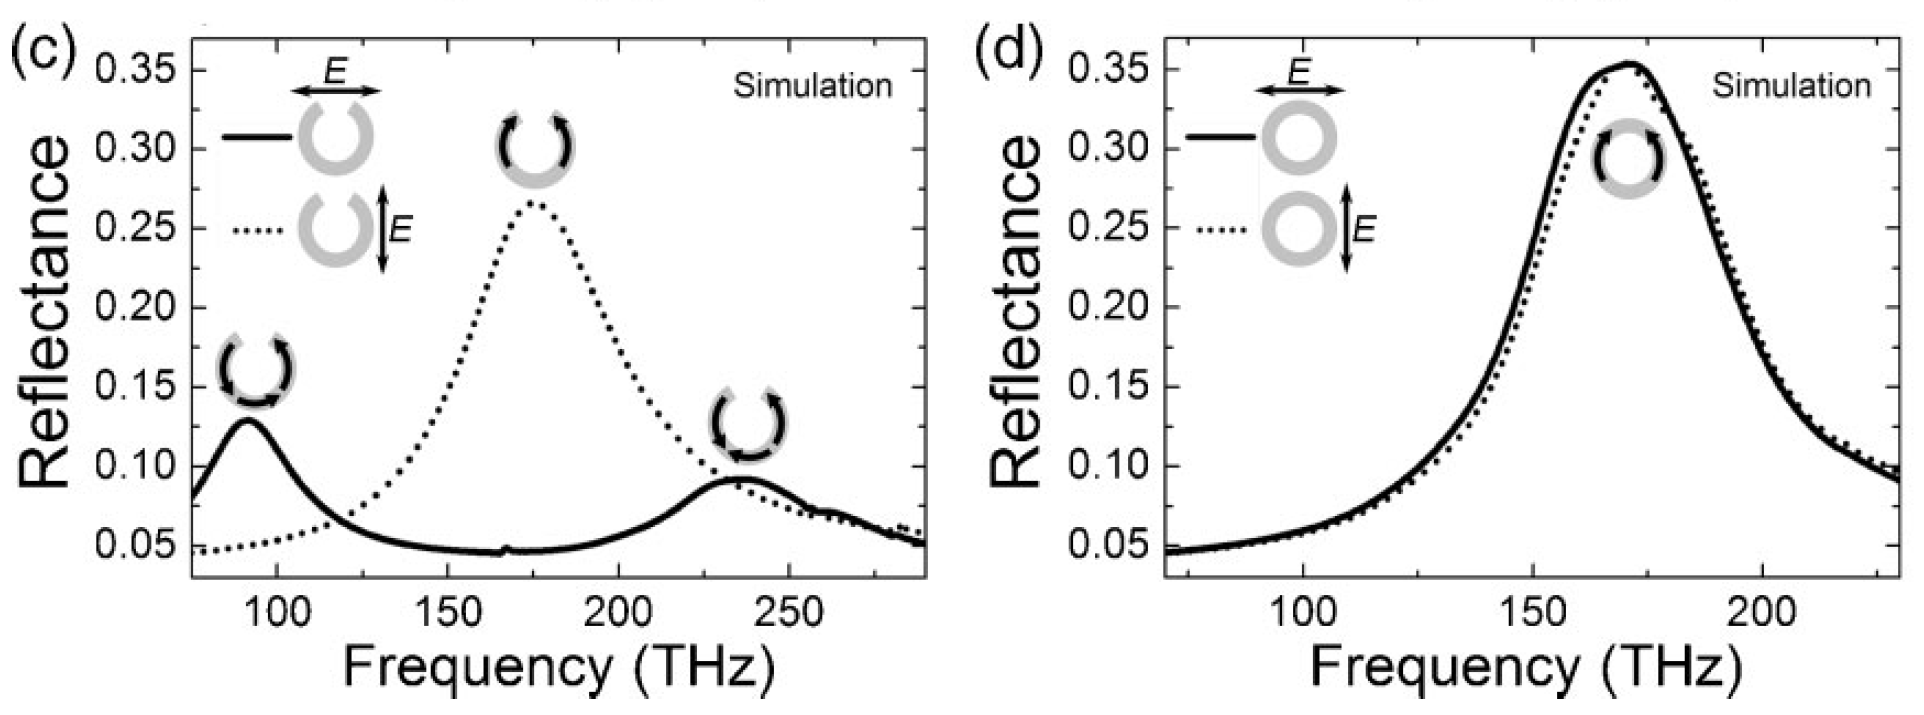
\includegraphics[scale=1]{../figures/spectrum_theory.png}
\caption{Simulated reflection spectrum of SRR and a full ring for different polarisations. \cite{paper_Giessen_meta}  }
    \label{spectrum_theory}
\end{figure}

    \end{block}    

    \begin{block}{\circled{3} Fabrication of a Monolayer Mask}
        \begin{figure}[htbp]
\begin{subfigure}[t][][t]{0.48\textwidth}
    \begin{tikzpicture}
    [x=0.1\textwidth, y=0.1\textwidth]
    \draw (0,0) rectangle (10,5);
    \draw[thick] (0.5,4.5) circle(0.3) node{1};
    \filldraw[orange]
        (1,2.2) .. controls (0.8,2.5) ..
        (1.2,3.5) .. controls (1.6,2.5) ..
        (1.4,2.2);
    \filldraw[red]
        (1.2,3) .. controls (1.4,2.5) ..
        (1.2,2.3) .. controls (1,2.5) ..
        (1.2,3);
    \draw[fill=darkgrey]
        (0.2,0.2)--
        (2.2,0.2)--
        (1.4,1.2)--
        (1.4,2.2)--
        (1,2.2)--
        (1,1.2)--
        (0.2,0.2);
    \draw[fill=brightgrey]
        (1.2,3.5)--
        (0.4,3.2)--
        (0.38,3.25)--
        (1.2,3.6)--
        (1.6,3.63)--
        (1.8,3.7)--
        (5,3.7)--
        (5,3.4)--
        (1.8,3.4)--
        (1.6,3.47)--
        (1.2,3.5);
    \filldraw[red,scale=0.5,shift={(11.5,7)}]
        (0,.5)--
        (2,.5)--
        (2,1)--
        (3,0)--
        (2,-1)--
        (2,-.5)--
        (0,-.5);
%    \draw[fill=red]
%        (4,1)--
%        (6,1)--
%        (6,0.5)--
%        (7,1.5)--
%        (6,2.5)--
%        (6,2)--
%        (4,2)--
%        (4,1);
    \draw[fill=brightgrey,shift={(8.5,4.5)}]
        (0,0)--
        (0.025,0.05)--
        (0.525,-0.2)..controls(0.6,-0.25)..
        (0.525,-0.3)--
        (-0.175,-0.65)--
        (-0.16,-1)--
        (-0.11,-1.1)--
        (-0.11,-4)--
        (-0.365,-4)--
        (-0.365,-1.1)--
        (-0.315,-1)--
        (-0.3,-0.65)..controls(-0.25,-0.6)..
        (-0.2,-0.57)--
        (0.48,-0.25)--
        (0,0);
     % text
     \draw[] (1.5,0.5)--(2.5,0.5) node[right]{Bunsen burner};
     \draw[] (2.5,3.5)--(2.5,2.9) node[right]{glass pipette};
     \draw[] (8.45,4.5)--(8,4.5) node[left]{reduce the size of the opening};
    \end{tikzpicture}
    \subcaption{Bending of a glass pipette through melting.}
\end{subfigure}
\hfill
\begin{subfigure}[t][][t]{0.48\textwidth}
    \begin{tikzpicture}
    [x=0.1\textwidth, y=0.1\textwidth]
    \draw (0,0) rectangle (10,5);
    \draw[thick] (0.5,4.5) circle(0.3) node{2};
    \filldraw[water] (0.5,0.5) rectangle (9.5,2.2);
    \draw[fill=grey]
        (0.2,2.5)--
        (0.5,2.5)--
        (0.5,0.5)--
        (9.5,0.5)--
        (9.5,2.5)--
        (9.8,2.5)--
        (9.8,0.2)--
        (0.2,0.2)--
        (0.2,2.5);
    \draw[fill=solution,shift={(5,1.5)},rotate=250,scale=1.2]
        (0,0)--
        (0.025,0.05)--
        (0.525,-0.2)..controls(0.6,-0.25)..
        (0.525,-0.3)--
        (-0.175,-0.65)--
        (-0.16,-1)--
        (-0.11,-1.1)--
        (-0.11,-4)--
        (-0.365,-4)--
        (-0.365,-1.1)--
        (-0.315,-1)--
        (-0.3,-0.65)..controls(-0.25,-0.6)..
        (-0.2,-0.57)--
        (0.48,-0.25)--
        (0,0);
    \draw[fill=brightgrey,shift={(5,1.5)},rotate=250,scale=1.2]
        (-0.11,-4)--
        (-0.11,-2)--
        (-0.365,-1.3)--
        (-0.365,-4)--
        (-0.11,-4);
    \draw[line width=0.006\textwidth,dotted,color=solution]
        (5.02,1.5) to[thick] (5.02,2.2);
    \foreach \i in {0.55,0.66,...,2.55}
        \filldraw[sphere] (\i,2.25) circle (0.05);
    \foreach \i in {7.45,7.56,...,9.45}
        \filldraw[sphere] (\i,2.25) circle (0.05);
    \draw[sphere,->,line width=0.007\textwidth]
        (5.2,1.5)..controls(5.2,2.2)and(5.35,2.25)..
        (7,2.25);
    % text
    \draw[] (9.65,2.5)--(9.65,4.5) node[left]{Petri dish};
    \draw[] (9.3,2.3)--(9.3,4) node[left]{microsphere monolayer};
    \draw[] (8.95,1.5)--(8.95,3.5) node[left]{destilled water};
    \draw[] (2.2,3.5) node[right]{particle solution};
    \draw[] (3.8,2.2)--(3.8,3.3);
    \end{tikzpicture}
    \subcaption{Creation of a microsphere monolayer at the water surface.}
\end{subfigure}

\begin{subfigure}[t][][t]{0.48\textwidth}
    \begin{tikzpicture}
    [x=0.1\textwidth, y=0.1\textwidth]
    \draw (0,0) rectangle (10,5);
    \draw[thick] (0.5,4.5) circle(0.3) node{3};
    \filldraw[water] (0.5,0.5) rectangle (9.5,1.44);
    \draw[fill=grey]
        (0.2,2.5)--
        (0.5,2.5)--
        (0.5,0.5)--
        (9.5,0.5)--
        (9.5,2.5)--
        (9.8,2.5)--
        (9.8,0.2)--
        (0.2,0.2)--
        (0.2,2.5);
    \foreach \i in {2.25,2.14,...,1.49}
        \filldraw[sphere] (0.55,\i) circle (0.05);
    \foreach \i in {0.55,0.66,...,5.55}
        \filldraw[sphere] (\i,1.49) circle (0.05);
    \draw[fill=substrate]
        (1,0.5) rectangle (2,.7)
        (3,0.5) rectangle (4,.7);
    \draw[sphere,->,ultra thick]
        (1.5,1.3) -- (1.5,0.8);
    \draw[sphere,->,ultra thick]
        (3.5,1.3) -- (3.5,0.8);
    \draw[ultra thick,fill=water]
        (8,1)..controls(8.5,3.8)..
        (10,4.5)--
        (10,4)..controls(9,3.5)..
        (8.5,1);
    \draw[ultra thick,->]
        (8.35,1.4)--(8.5,2.12);
    % text
    \draw[] (9.6,4)--(9,4.5) node[left]{suck away the water through the hose};
    \draw[] (1.8,0.6)--(1.8,3.5) node[right]{substrate};
    \draw[] (2.5,1.5)--(2.5,2.5) node[right]{monolayer subsides};
    \end{tikzpicture}
    \subcaption{Applying the monolayer to the substrates.}
\end{subfigure}
\hfill
\begin{subfigure}[t][][t]{0.48\textwidth}
    \begin{tikzpicture}
    [x=0.1\textwidth, y=0.1\textwidth]
    \draw (0,0) rectangle (10,5);
    \draw[thick] (0.5,4.5) circle(0.3) node{4};
    \draw[fill=substrate]
        (0.5,0.5) rectangle (2.5,0.7)
        (0.5,1.5) rectangle (2.5,3.5);
    \foreach \i in {1.63,1.9764,...,3.41}
        \foreach \j in {0.6,0.8,...,2.41}
            \filldraw[sphere] (\j,\i) circle (0.095);
    \foreach \i in {1.8032,2.1496,...,3.41}
        \foreach \j in {0.7,0.9,...,2.41}
            \filldraw[sphere] (\j,\i) circle (0.095);
    \foreach \i in {0.6,0.8,...,2.41}
        \filldraw[sphere] (\i,0.795) circle (0.095);
    \coordinate (s) at (7,0);
    \draw[fill=substrate,shift={(s)}]
        (0.5,0.5) rectangle (2.5,0.7)
        (0.5,1.5) rectangle (2.5,3.5);
    \foreach \i in {1.63,1.9764,...,3.41}
        \foreach \j in {0.6,0.8,...,2.41}
            \filldraw[sphere,shift={(s)}] (\j,\i) circle (0.105);
    \foreach \i in {1.8032,2.1496,...,3.41}
        \foreach \j in {0.7,0.9,...,2.41}
            \filldraw[sphere,shift={(s)}] (\j,\i) circle (0.105);
    \foreach \i in {0.6,0.8,...,2.41}
        \filldraw[sphere,shift={(s)}]
            (\i,0.79) ellipse [x radius=0.105,y radius=0.09];
    \filldraw[sphere]
        (4,1.3) ellipse [x radius=.5,y radius=.5]
        (6,1.25) ellipse [x radius=.55,y radius=.45];
    \draw[fill=substrate]
        (3.3,0.5) rectangle (4.7,0.8)
        (5.3,0.5) rectangle (6.7,0.8);
    \filldraw[red,yscale=.8,shift={(3.5,3.5)}]
        (0,.5)--
        (2,.5)--
        (2,1)--
        (3,0)--
        (2,-1)--
        (2,-.5)--
        (0,-.5);
    % text
    \draw[red] (3.5,3.6) node[right]{\SI{108}{\degreeCelsius}};
    \draw[red] (3.5,4.1) node[right]{$\SI{120}{\second}-\SI{240}{\second}$};
    \draw[] (1.5,3.5) node[above]{spheres};
    \draw[] (8.5,3.5) node[above]{ellipsioids};
    \draw[] (2.5,0.8)--(3.5,1.3);
    \draw[] (7.5,0.8)--(6.55,1.25);
    \end{tikzpicture}
    \subcaption{Annealing of the probe shrinks the space between the spheres.}
\end{subfigure}
\end{figure}

\begin{figure}[htbp]
\begin{minipage}[t][][t]{0.48\textwidth}
    Hier k\"onnte ihre Werbung stehen!
\end{minipage}
\hfill
\begin{subfigure}[t][][b]{0.48\textwidth}
    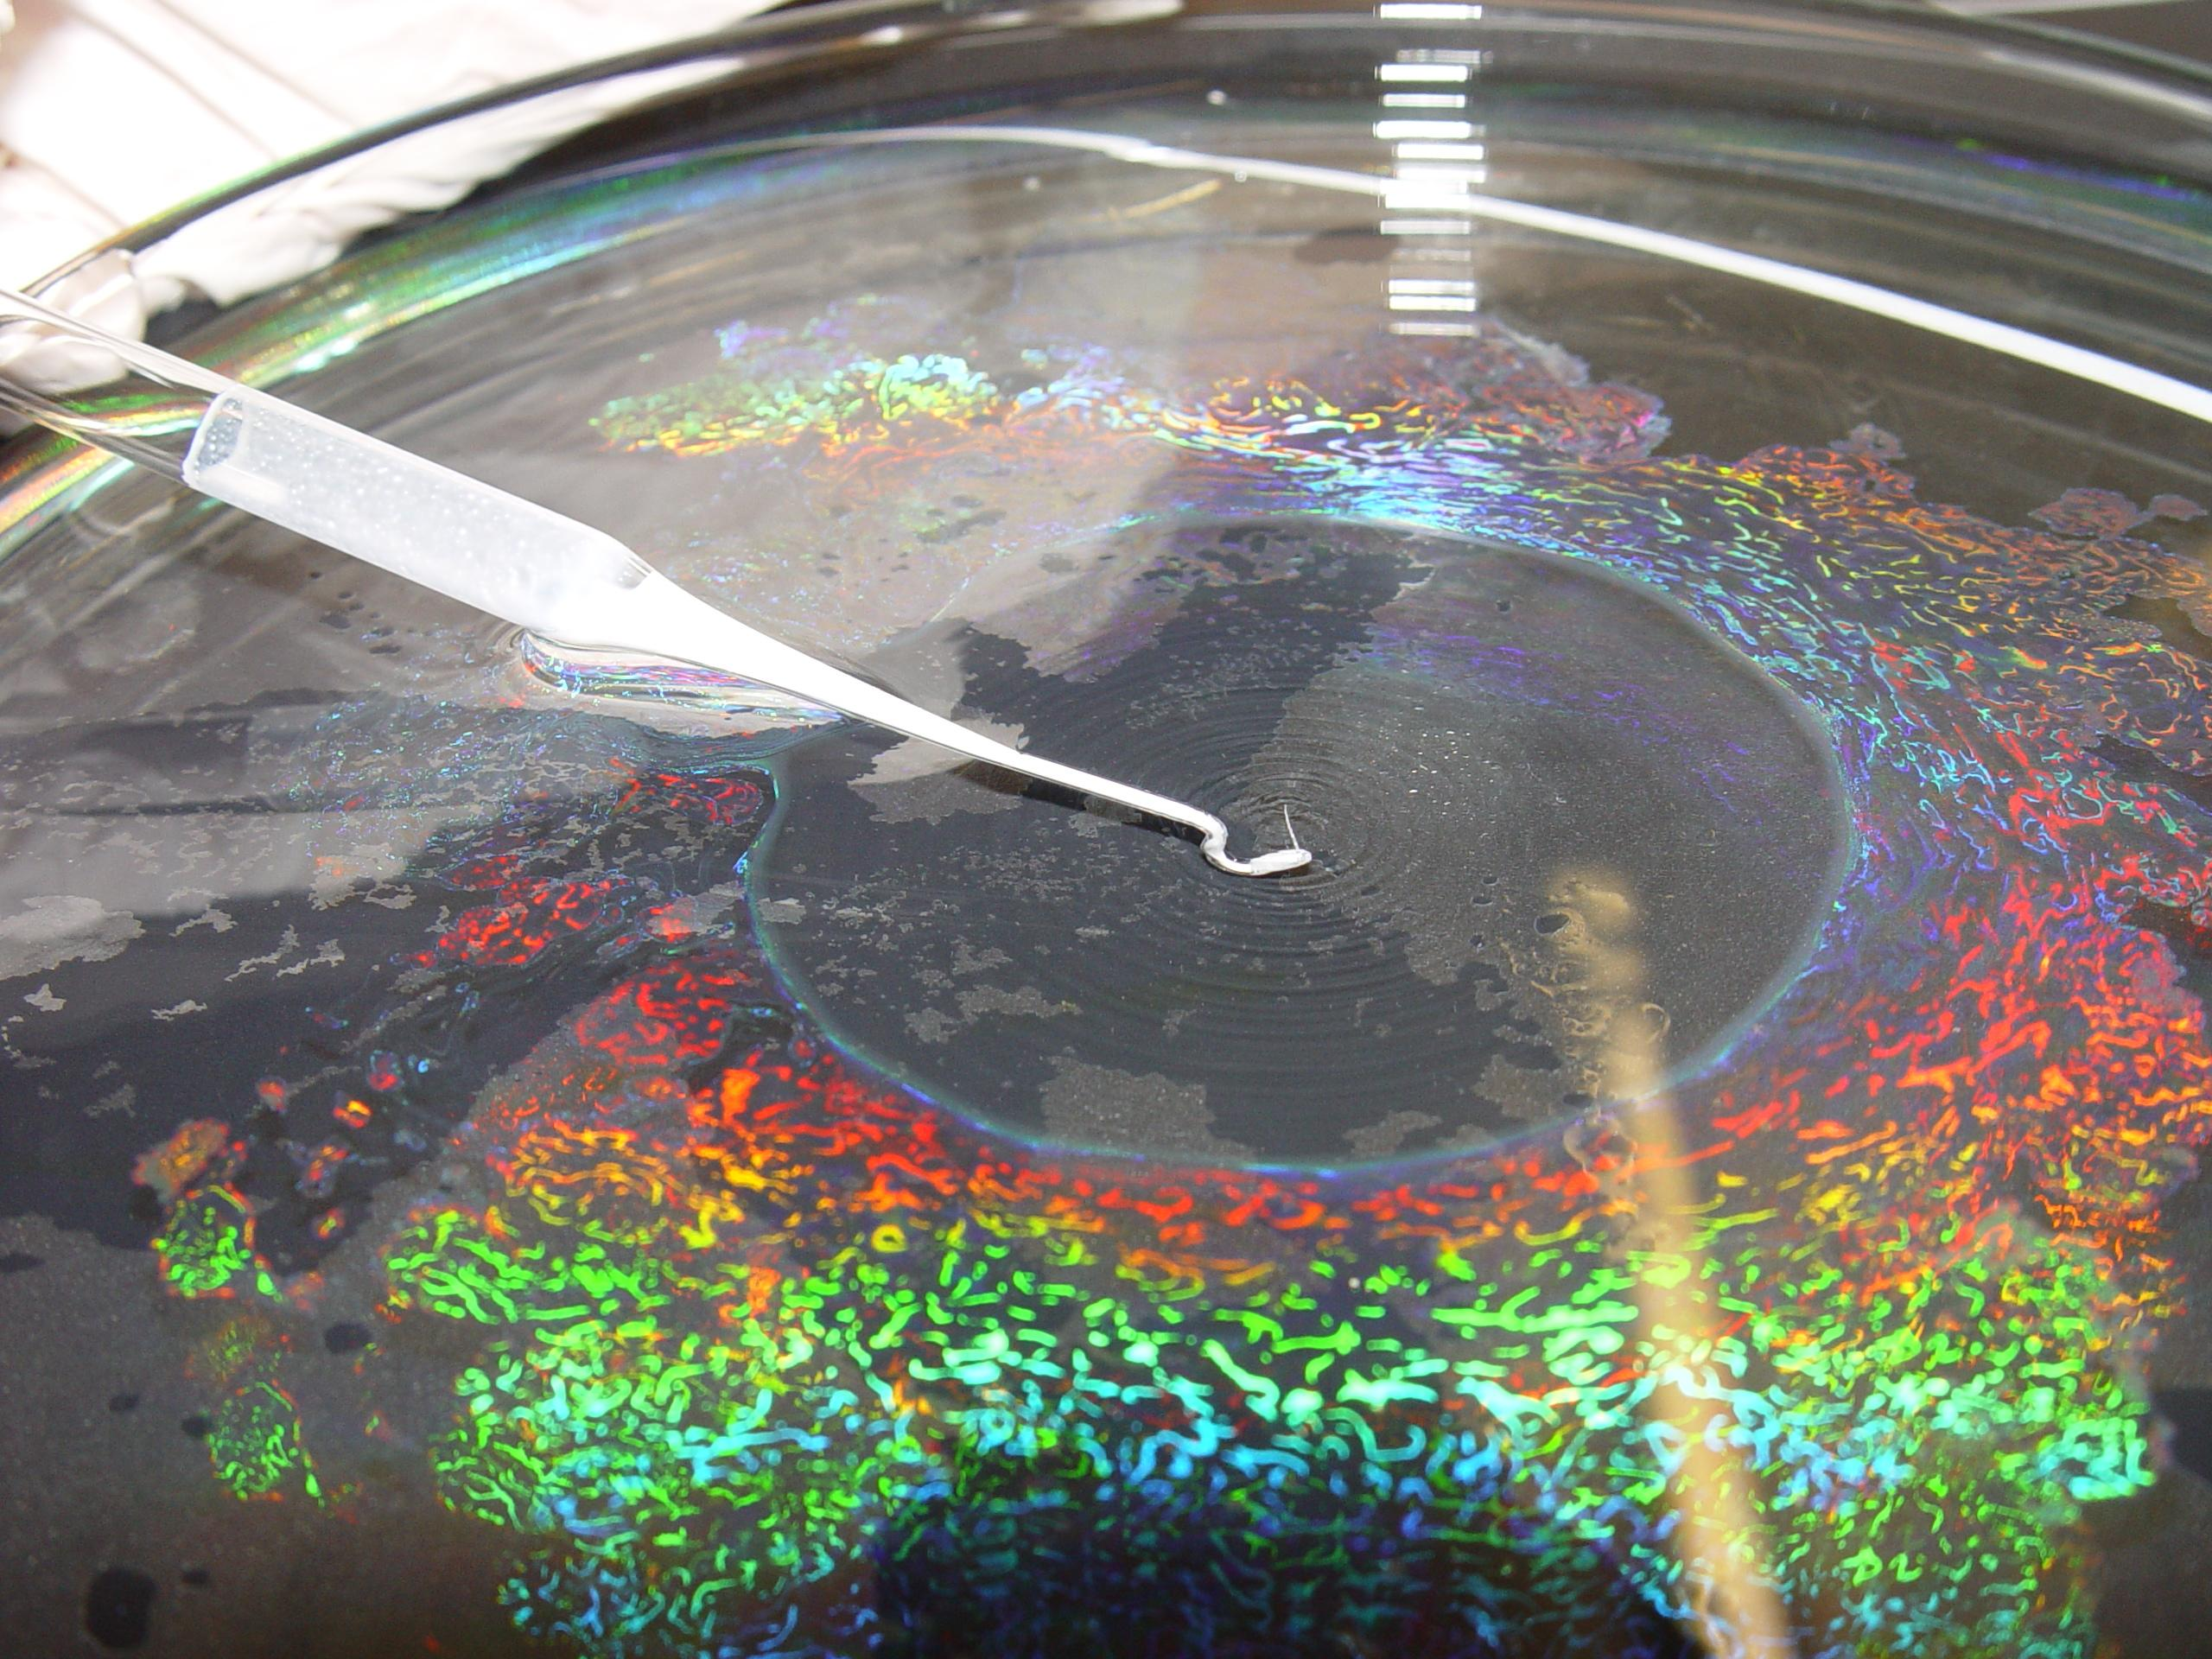
\includegraphics[width=\textwidth]{petrischale.jpg}
    \caption{Photography of (2).
        One can see the monolayer as shiny film.}
\end{subfigure}
\end{figure}
    \end{block}
    
     \begin{block}{\circled{4} Evaporation}
        The mask on the glass substrate is placed in the evaporating machine with a specific angle. Depending on the rotation of the mask during the evaporation can be created SRRs and full rings. 
\begin{figure}[H]
\centering
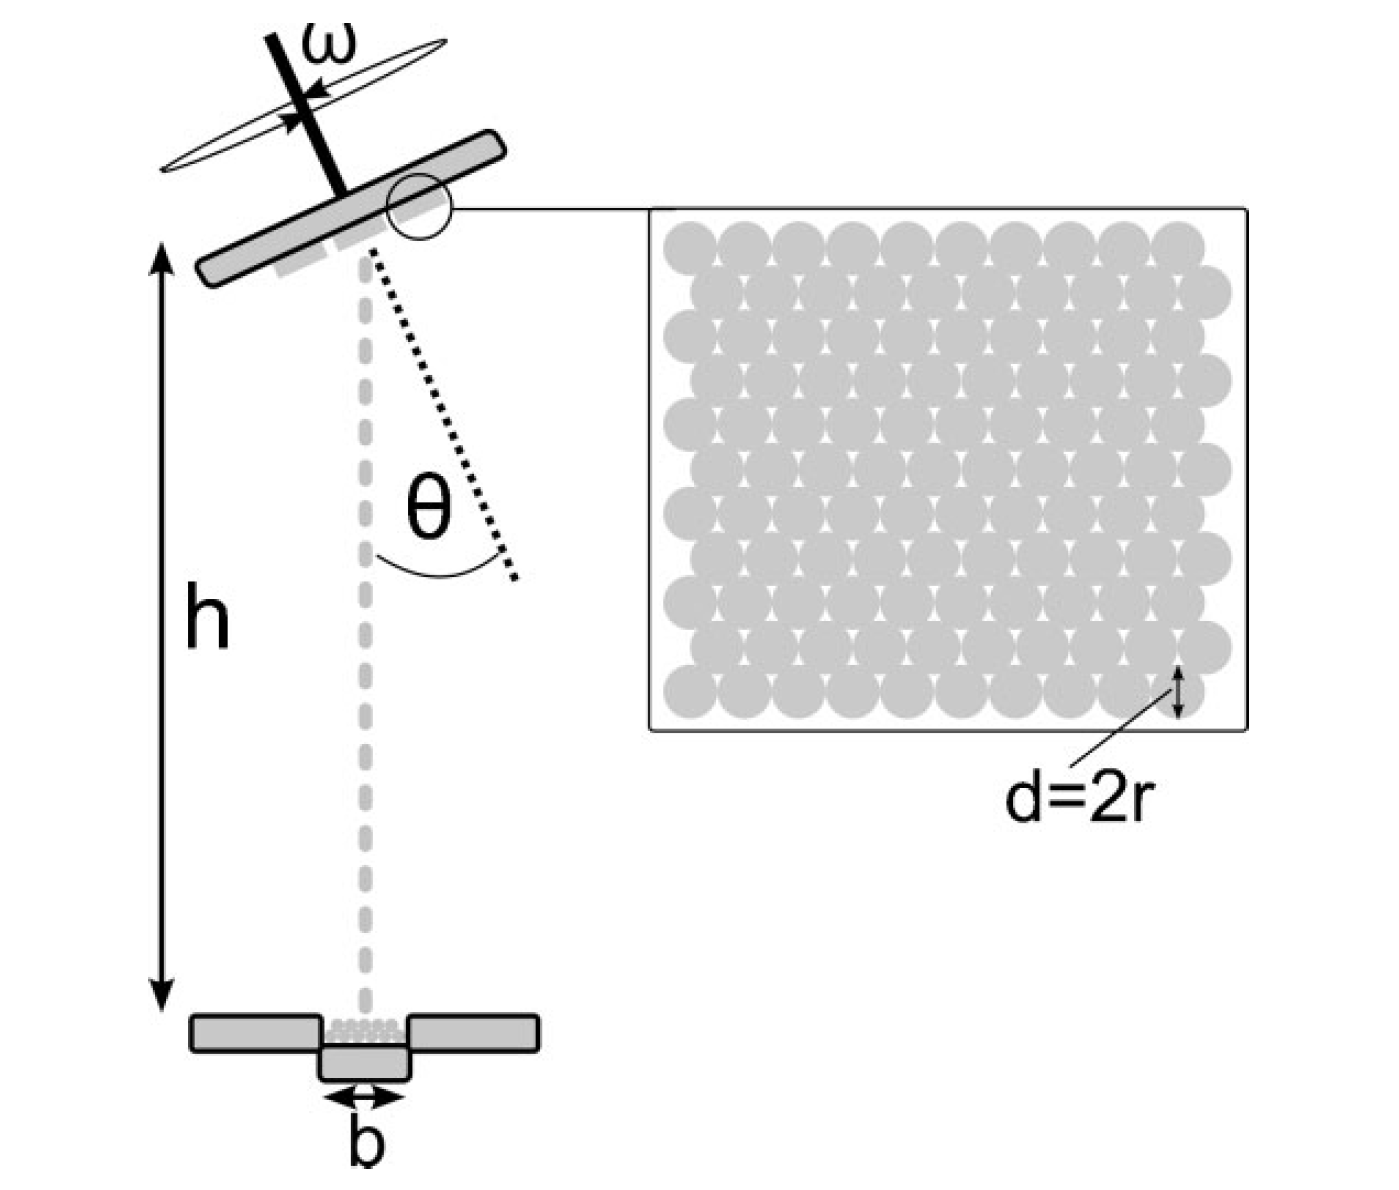
\includegraphics[scale=1]{../figures/evaporation.png}
\caption{Schematic drawing of the evaporating. \cite{paper_Giessen_meta}  }
    \label{spectrum_theory}
\end{figure}

     \end{block}
     
\end{column}

\begin{column}{0.48\linewidth}
    \begin{block}{Literature}
        \bibliography{mybib}{}
    \end{block}
\end{column}

\end{columns}
\end{frame}
\end{document}
